
\documentclass{article}
\usepackage[utf8]{inputenc}
\usepackage{relsize}
\usepackage{amsmath}
\usepackage{geometry}
\usepackage{tikz}
\usetikzlibrary{automata, positioning, arrows}
\tikzset{node distance=2.5cm, % Minimum distance between two nodes. Change if necessary.
every state/.style={ % Sets the properties for each state
semithick,
fill=gray!10},
initial text={}, % No label on start arrow
double distance=2pt, % Adjust appearance of accept states
every edge/.style={ % Sets the properties for each transition
draw,->,>=stealth', % Makes edges directed with bold arrowheads
auto,semithick}}

\geometry{
 a4paper,
 total={170mm,257mm},
 left=20mm,
 top=20mm,
}

\title{Homework 4\\[0.2em]\smaller{}CSC 445-01: Theory of Computation}
\author{Matthew Mabrey, Luke Kurlandski}
\date{\today}

\begin{document}

\maketitle

\section*{2.1}

% Parse tree generator https://yohasebe.com/rsyntaxtree/

\subsection*{a}
The parse tree for $a$ is
\begin{center}
    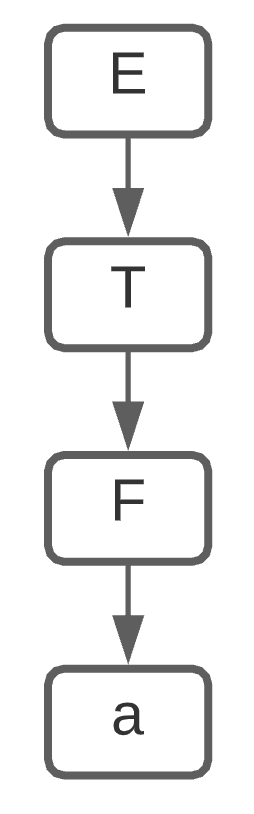
\includegraphics[scale=.65]{2.1.a.png}
\end{center}
The derivation for $a$ is
$$E \Rightarrow T \Rightarrow F \Rightarrow a$$

\pagebreak

\subsection*{b}
The parse tree for $a+a$ is
\begin{center}
    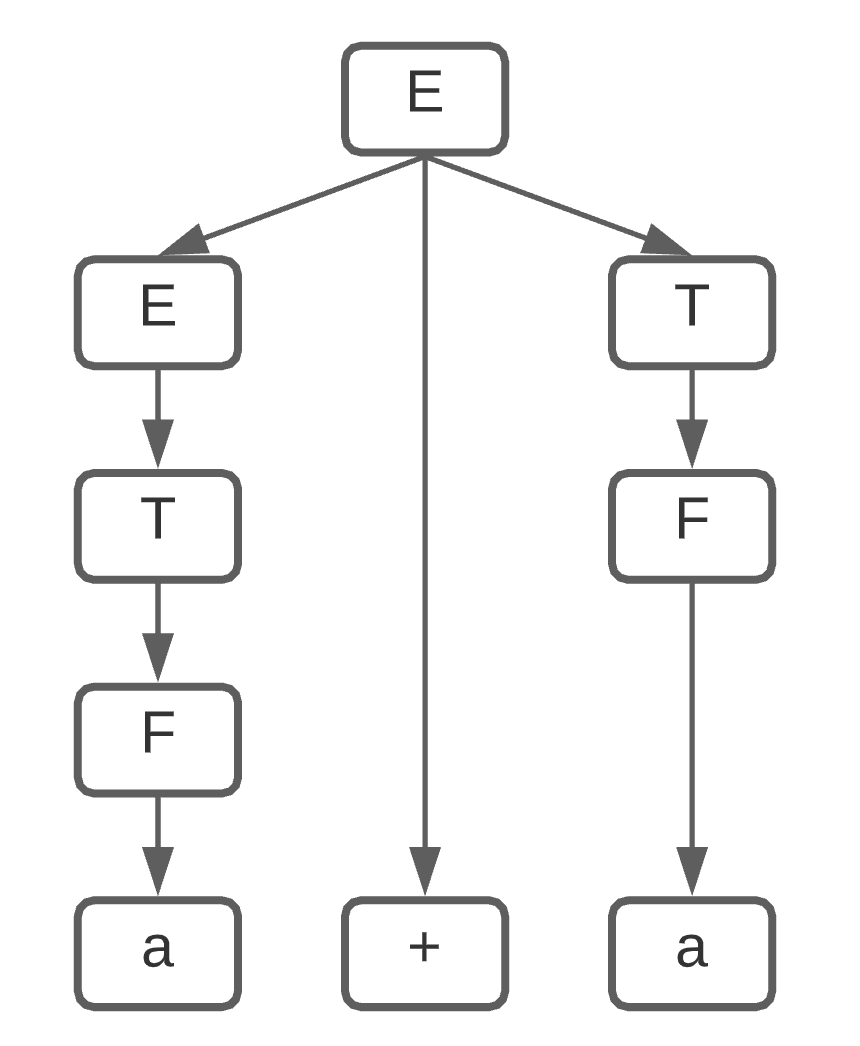
\includegraphics[scale=.65]{2.1.b.png}
\end{center}
The derivation for $a+a$ is
$$E \Rightarrow E+T \Rightarrow T+T \Rightarrow F+T \Rightarrow a + T \Rightarrow a + F \Rightarrow a + a$$

\pagebreak

\subsection*{c}
The parse tree for $a+a+a$ is
\begin{center}
    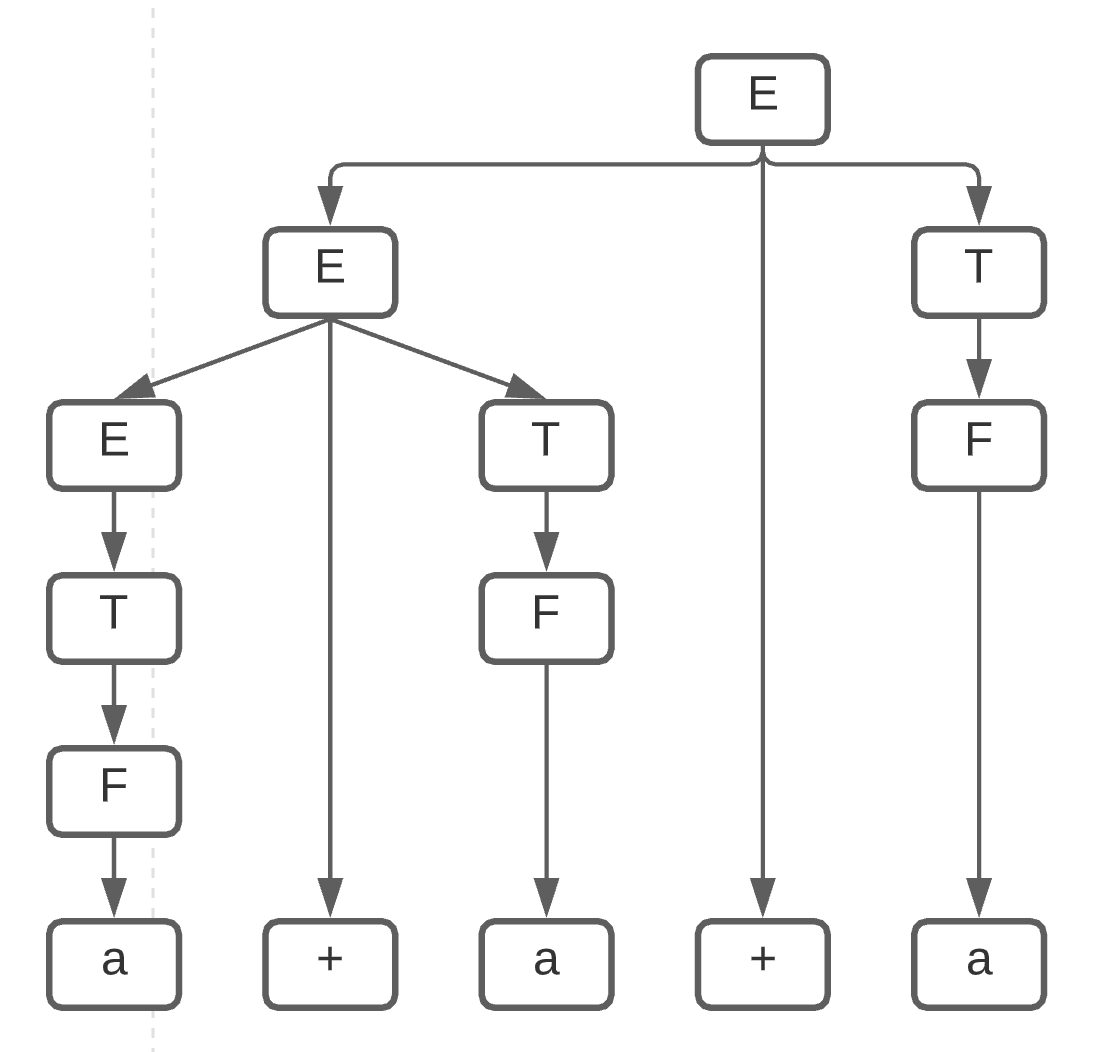
\includegraphics[scale=.65]{2.1.c.png}
\end{center}
The derivation for $a+a+a$ is
\begin{align*}
    E &\Rightarrow E+T \Rightarrow E + T+ T \Rightarrow T+T+T \Rightarrow F + T + T \Rightarrow a + T + T \\
    & \Rightarrow a + F + T \Rightarrow a + a + T \Rightarrow a + a + F \Rightarrow a+a+a
\end{align*}

\pagebreak

\subsection*{d}
The parse tree for $((a))$ is
\begin{center}
    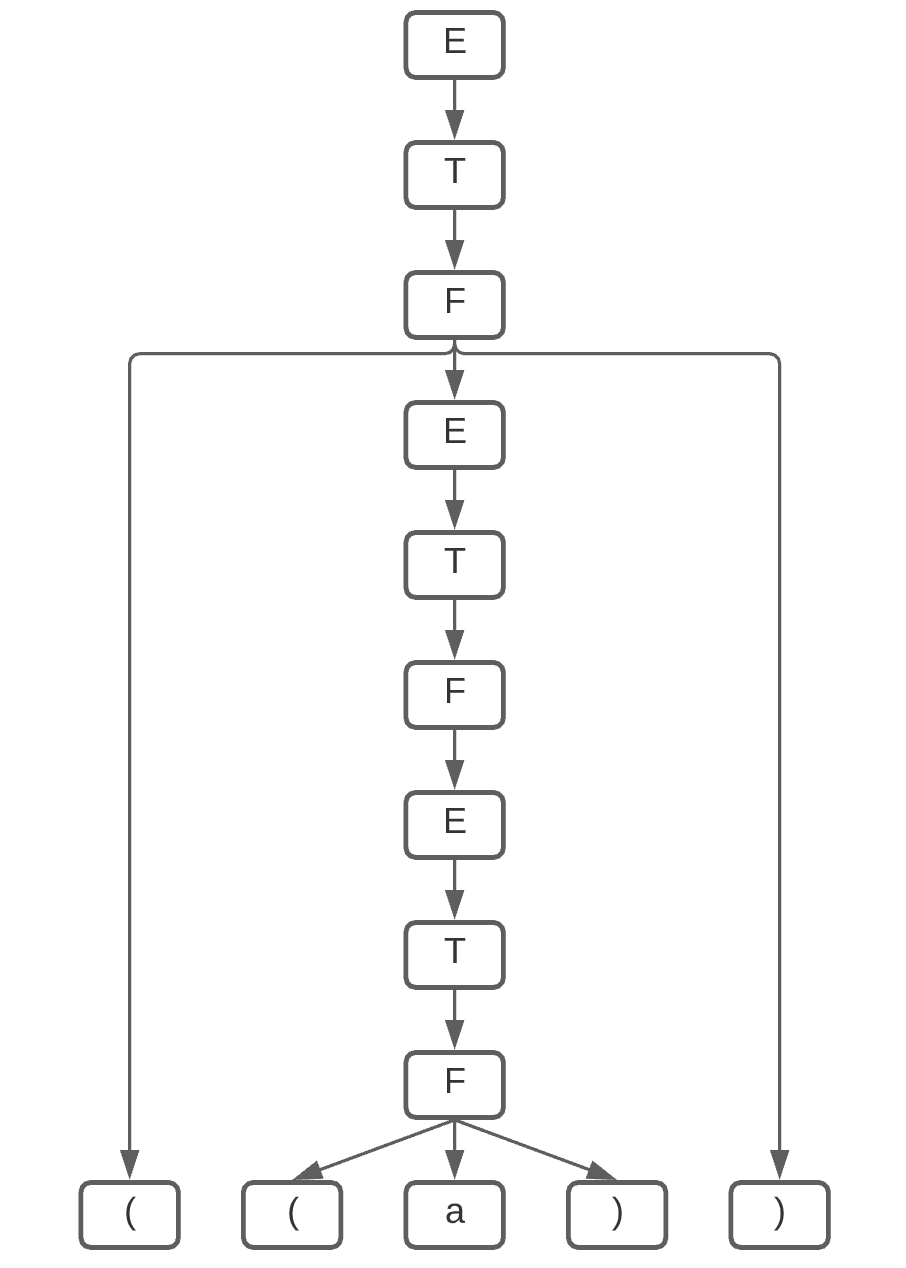
\includegraphics[scale=.65]{2.1.d.png}
\end{center}
The derivation for $((a))$ is
\begin{align*}
    E \Rightarrow T \Rightarrow F \Rightarrow(E) \Rightarrow (T) \Rightarrow (F) \Rightarrow ((E)) \Rightarrow ((T)) \Rightarrow ((F)) \Rightarrow((a))
\end{align*}

\pagebreak

\section*{2.4}

\section*{2.5}

\subsection*{b}
% Tests this PDA: {"type":"PDA","pda":{"transitions":{"start":{"0":{"":[{"state":"s0","stackPushChar":"0"},{"state":"s1","stackPushChar":""}]},"1":{"":[{"state":"s0","stackPushChar":"1"},{"state":"s1","stackPushChar":""}]}},"s0":{"0":{"0":[{"state":"s1","stackPushChar":""}],"":[{"state":"s0","stackPushChar":""}]},"1":{"1":[{"state":"s1","stackPushChar":""}],"":[{"state":"s0","stackPushChar":""}]}}},"startState":"start","acceptStates":["s1"]},"states":{"start":{},"s0":{"top":170,"left":279,"displayId":"s0"},"s1":{"isAccept":true,"top":258,"left":584,"displayId":"s1"}},"transitions":[{"stateA":"start","label":"0,ϵ,0","stateB":"s0"},{"stateA":"start","label":"0,ϵ,ϵ","stateB":"s1"},{"stateA":"start","label":"1,ϵ,1","stateB":"s0"},{"stateA":"start","label":"1,ϵ,ϵ","stateB":"s1"},{"stateA":"s0","label":"0,0,ϵ","stateB":"s1"},{"stateA":"s0","label":"0,ϵ,ϵ","stateB":"s0"},{"stateA":"s0","label":"1,1,ϵ","stateB":"s1"},{"stateA":"s0","label":"1,ϵ,ϵ","stateB":"s0"}],"bulkTests":{"accept":"0\n1\n00\n11\n101\n1001\n010\n0110\n0101010\n1010001101\n0111110\n0110101010\n00000010\n100000011111","reject":"\n10\n01\n001\n110\n1010\n0101\n1010010\n01101\n01010101\n10100011010"}}

\subsection*{e}

% Test this PDA:      {"type":"PDA","pda":{"transitions":{"start":{"E":{"E":[]},"":{"":[{"state":"s0","stackPushChar":"$"}]}},"s0":{"0":{"E":[],"":[{"state":"s1","stackPushChar":""},{"state":"s0","stackPushChar":"0"}]},"1":{"E":[],"":[{"state":"s1","stackPushChar":""},{"state":"s0","stackPushChar":"1"}]},"E":{"E":[]},"":{"":[{"state":"s1","stackPushChar":""}]}},"s1":{"0":{"0":[{"state":"s1","stackPushChar":""}]},"1":{"1":[{"state":"s1","stackPushChar":""}]},"E":{"$":[]},"":{"$":[{"state":"s2","stackPushChar":""}]}}},"startState":"start","acceptStates":["s2","start"]},"states":{"start":{"isAccept":true},"s0":{"top":92,"left":395,"displayId":"s0"},"s1":{"top":401,"left":395,"displayId":"s1"},"s2":{"isAccept":true,"top":400,"left":4,"displayId":"w=w^R"}},"transitions":[{"stateA":"start","label":"ϵ,ϵ,$","stateB":"s0"},{"stateA":"s0","label":"0,ϵ,ϵ","stateB":"s1"},{"stateA":"s0","label":"0,ϵ,0","stateB":"s0"},{"stateA":"s0","label":"1,ϵ,ϵ","stateB":"s1"},{"stateA":"s0","label":"1,ϵ,1","stateB":"s0"},{"stateA":"s0","label":"ϵ,ϵ,ϵ","stateB":"s1"},{"stateA":"s1","label":"0,0,ϵ","stateB":"s1"},{"stateA":"s1","label":"1,1,ϵ","stateB":"s1"},{"stateA":"s1","label":"ϵ,$,ϵ","stateB":"s2"}],"bulkTests":{"accept":"\n101\n010\n0000\n1111\n01010\n10101\n001100\n110011","reject":"10\n01\n1010\n0101\n10101001001\n110001\n1101010011"}}

Begin by placing $\$$ on the stack. Read input and push the input symbols on the stack. This first phase is symbolic of reading the first half of the string. Nondeterministically, at some point of reading input, start comparing input symbols with symbols popped from the stack. If input symbol and stack symbol do not match, halt without accepting, else, continue. This second phase is symbolic of reading the second half of the string and checking that it matches the first half. Our PDA carefully handles this transition to account for even/odd numbered strings. Finally, if input symbol is $\epsilon$ and stack symbol is $\$$, halt and accept. 

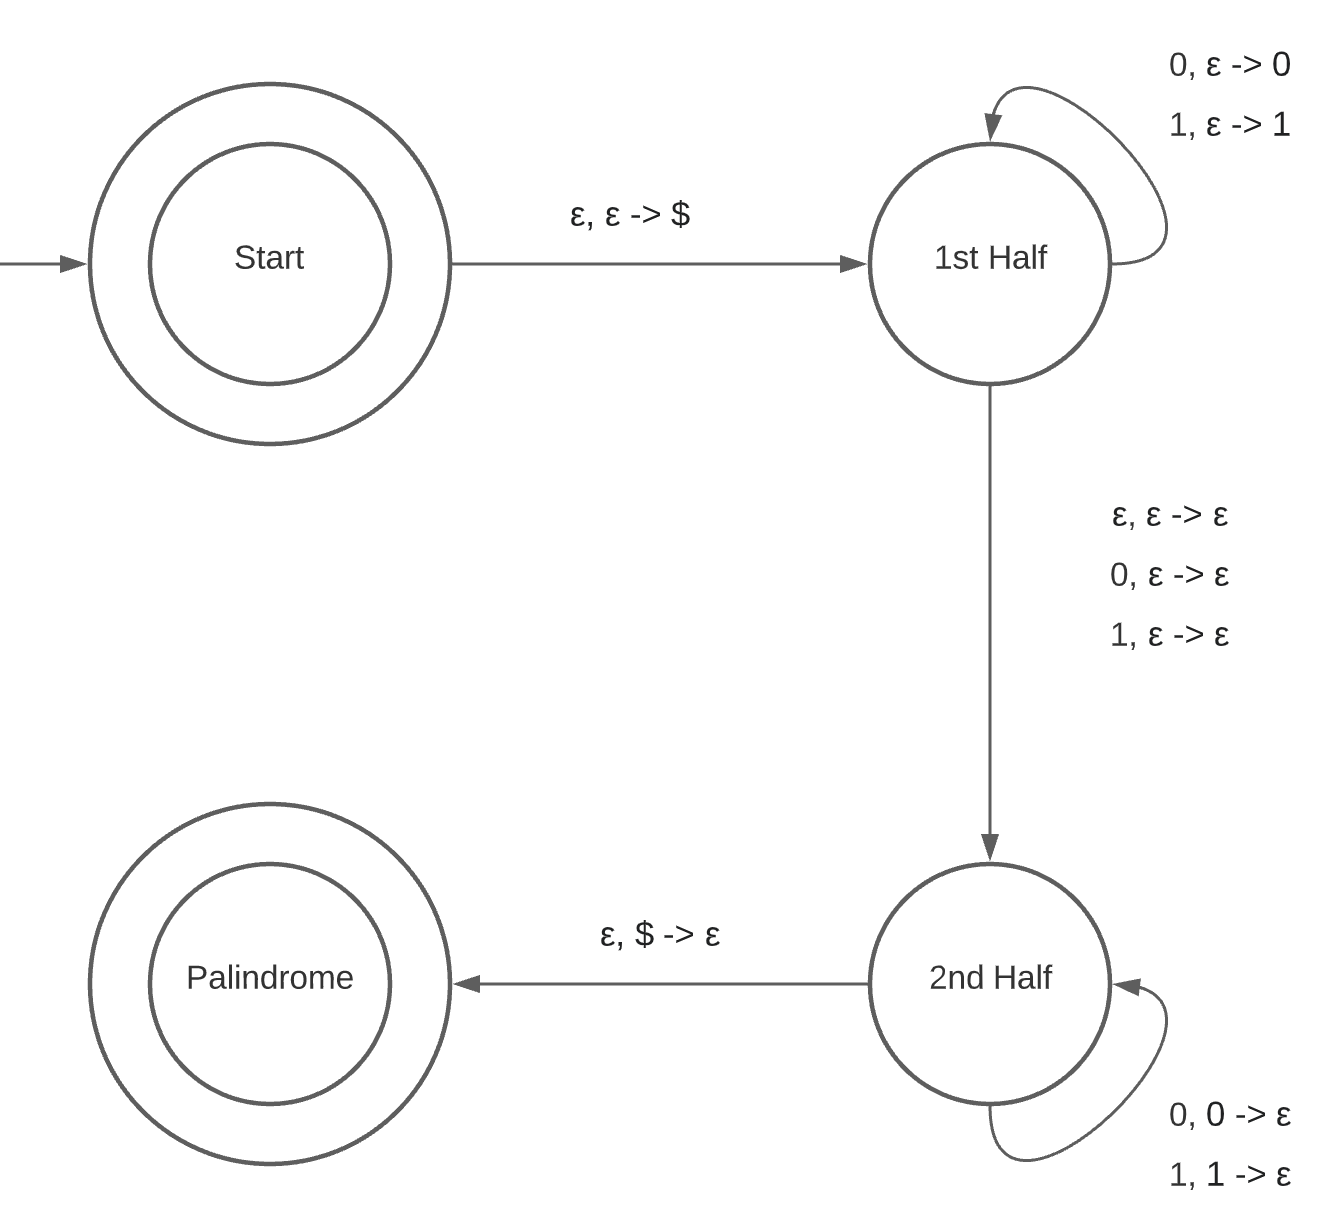
\includegraphics[scale=.65]{2.5.b.png}

\section*{2.6}

\section*{2.13}

This grammar may produce a string that belongs to one of two different languages. The first language is that of zero or more $0$s, followed by a $\#$, followed by two times as many $0$s that came before. The second language is that of zero or more $0$s, followed by a $\#$, followed by zero or more $0$s, followed by a $\#$, followed by zero or more $0$s.\\\\
More formally,
$$L(G) = \{ 0^n\#0^{2n} \; | \; n \geq 0 \} \cup  \{ 0^a\#0^b\#0^c \; | \; a,b,c \geq 0 \}$$

\end{document}
